\chapter{A Novel Readout Technique for TPCs: Q-Pix}~\label{chap:qpix}

We begin this chapter in Section~\ref{sec:qpix_circuit} by introducing a novel pixel-based readout concept for TPCs.
Pixel-based readouts offer several advantages over the traditional wire readout \citep{lartpc_recon_problems_joshi_2015}.
A key improvement offered by pixelization is true 3-D image reconstruction.
This allows for sharper vertex reconstruction, improving the overall resolution of of a LArTPC and may reduce the time required for a NP measurement.
Other benefits include a reduction in the amount of data storage required and there simpler data analysis.

Next, in Section~\ref{sec:qpix_apa} we discuss how this readout technology can be extended to a DUNE-FD 10 kT module.
We compare the design specifications for the current wire-based readout of a DUNE-FD and discuss how the Q-Pix readout can meet similar design goals.
We note the advantages of pixelization come at the cost of increased design complexity.
The traditional wire-based readout of a DUNE-FD module will have hundreds to thousands of channels, while a pixel-based readout will have tens of millions of channels.
This number of channels required to provide a stable readout over the expected lifetime of DUNE ($\approx 20$ years), where the electronics are continuously operating at liquid argon temperatures.
A goal of this dissertation is to address the channel size problem.

Two prototype ASICs have been developed to test each side of the readout shown in Figure~\ref{fig:qpix_frontandbackend}.
We refer to the ASIC developed to test the front-end as the "analog ASIC".
Likewise, we refer to the ASIC developed to test the back-end as the "digital ASIC".
The contributions to the design of digital ASIC is a major component of this thesis.
In Section~\ref{sec:digital_back-end} we discuss the design challenges of a large pixelated detector, with a special emphasis on the requirements of the digital back-end.
Finally, in Sections~\ref{sec:qpix_photonics} and~\ref{sec:qpix_supernova} we briefly describe other work towards validating the Q-Pix design in a LArTPC.

\section{Q-Pix: The Circuit Level Design}~\label{sec:qpix_circuit}

The fundamental Q-Pix circuit~(\ref{fig:qpixCircuit}) was first introduced by Nygren and Mei~\citep{qpix:nygren:mei}.
The principle of the front-end circuit operates on producing a signal output from Schmitt trigger connected to a charge sensitive amplifier (CSA) circuit.
The CSA's input is connected to the anode of a TPC where drifted electron charge accumulates.
Voltage is then built up across the capacitor from the accumlating charge according to the equation:

\begin{equation}~\label{eq:capacitor}
Q_{i} = C_{i}V_{i}
\end{equation}

After the capacitor voltage exceeds a set threshold ($V_{i}$) the schmitt trigger activates.
The Schmitt trigger output is sent as a signal input to the digital logic to be recorded.
This signal is shown as the output in Figure~\ref{fig:qpixCircuit}.
The Schmitt trigger input to the digital back-end is recorded against a free running local oscillator ($f_{o} = 30~\unit{MHz}$ ).

\begin{figure}[]
\centering
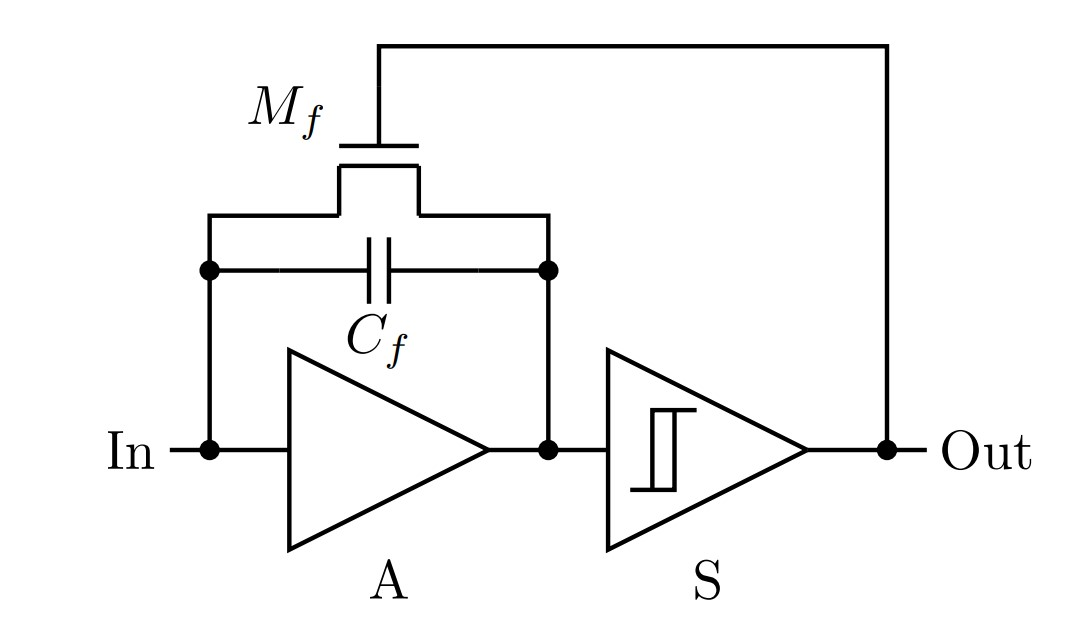
\includegraphics[width=\textwidth]{images/qpix_circuit.jpg}
\caption{A simplified schematic of front-end Q-Pix Readout circuit.
The front-end is a charge sensitive amplifier (CSA) whose output is connected to a Schmitt trigger.
The trigger (output) occurs when enough charge as accumulated on the capacitor $C_{f}$ (currently 1~\unit{fC}).
One of the design parameters for the Q-Pix front-end is the choice of $C_{f}$.
This front-end circuit is designed within a single analog ASIC which has contains 16 of these circuits.
The schematic for this ASIC is shown in Apendix~\ref{app:analog_prototype}.
Image is taken from~\citep{qpix:nygren:mei}.}
\label{fig:qpixCircuit}
\end{figure}

The Q-Pix readout records 32-bit latch values as a response to the Schmitt trigger output; it does not measure voltage, charge, or time.
We refer to this 32-bit measurement as a "timestamp".
These timestamps are produced when enough charge accumlates on the capacitor to produce a reset pulse, therefore the Q-Pix readout does not depend on an external system trigger to acquire data.

There are two components of the Q-Pix readout: analog and digital.
The analog portion of the readout begins with the CSA and ends at the Schmitt trigger output.
The digital portion of the readout begins at timestamp record.
These two portions are shown in Figure~\ref{fig:qpix_frontandbackend}.

\begin{figure}[]
\centering
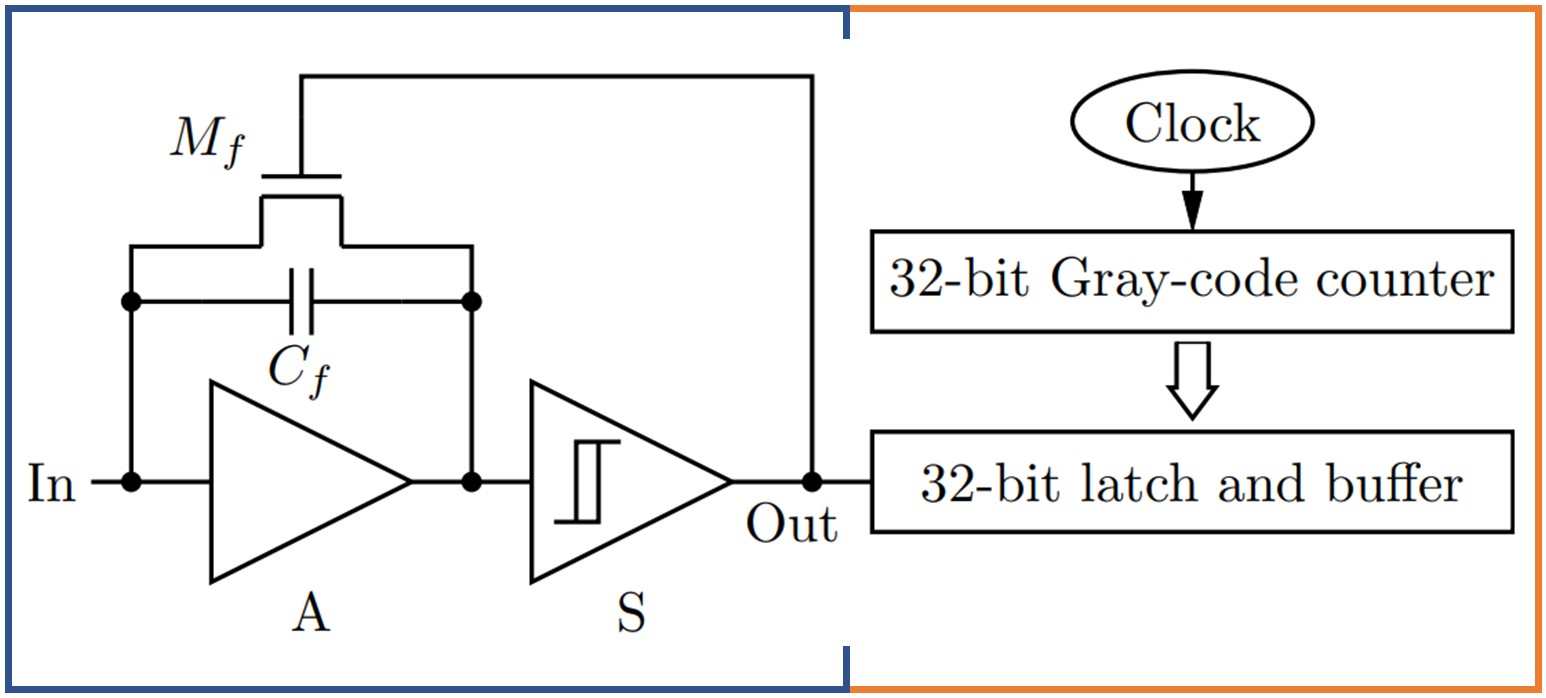
\includegraphics[width=\textwidth]{images/qpix_circuit_frontandbackend.jpg}
\caption{A modified image from~\citep{qpix:nygren:mei} is shown.
The blue box is the Q-Pix circuit~(Figure~\ref{fig:qpixCircuit}), which we refer to as the Q-Pix "analog front-end".
The right side of the image, encompassed in orange box, we refer to as the "digital back-end".
The back-end is responsible for providing the local oscillator as well as accurately recording a reference counter to correspond to the time when the Schmitt trigger signal is received.
}
\label{fig:qpix_frontandbackend}
\end{figure}

\subsection{Current Reconstruction}~\label{sec:rtds_and_waveforms}

Here we describe the basic principle of reconstructing the input current from a collection of timestamp measurements.

A timestamp measurement indicates that a certain amount of charge was accumlated at the CSA.
Since total charge is conserved we can say that the total accumulated charge ($Q_{in}(t)$) is equal total amount of charge discharged from each reset ($Q_{out}(t)$) plus any residual charge still on the pixel ($Q_{c}(t)$).
Therefore, we can relate the total accumulated charge to the total charge discharged with the following equation:

\begin{equation}~\label{eq:qin}
Q_{in}(t) = Q_{out}(t) + Q_{c}(t)
\end{equation}

One of the features of the analog ASIC is the replishment circuit.
This circuit is a constant current source which can remove a constant number of electrons from the CSA.
This provides a major simplification to the current reconstruction.
If we assume that each reset removes the same amount of charge ($Q_{o}$) we can rewrite the total charge out ($Q_{out}$) in terms of the integer number of resets at time t, ($N(t)$):

\begin{equation}~\label{eq:qout}
Q_{out}(t) = Q_{o} N(t)
\end{equation}

Equation~\ref{eq:qout} then gives us the measured current by definition ($I_{out} = \frac{dQ_{out}}{dt}$):
\begin{equation}~\label{eq:irecon}
I_{out} = \frac{d}{dt}(Q_{o}N(t)) = Q_{o}\frac{dN}{dt}
\end{equation}

We identify $\frac{dN}{dt}$ at the number of resets per unit time.
We can calculate the average current between two resets, or $\frac{dN}{dt} = \frac{1}{dT}$.
Then, $dT$ is the time difference between two resets and is measured at the local oscillator: $dT = \frac{f_{o}}{N_{rtd}}$, where $N_{rtd}$ is the difference between the two timestamps.
Equation~\ref{eq:irecon} becomes:

\begin{equation}~\label{eq:irecon_freq}
\boxed{I_{out} = \frac{Q_{o}f_{o}}{N_{rtd}}}
\end{equation}

Equation~\ref{eq:irecon_freq} shows the fundamental equation for the Q-Pix readout reconstruction.
There are three important parameters: the charge per reset ($Q_{o}$), the frequency of each local oscillator ($f_{o}$), and $N_{rtd}$ which is the difference between two timestamp measurements.
Figures which demonstrate the transistor level effects of this reconstruction are shown in Figures~\ref{fig:qpixRecon1} and~\ref{fig:qpixRecon2}.
Figures~\ref{fig:qpixRecon1} and~\ref{fig:qpixRecon2} show the charge reconstructions with a $Q_{o}$ value of 1~\unit{fC} and 0.3~\unit{fC}, respectively.

\begin{figure}[]
\centering
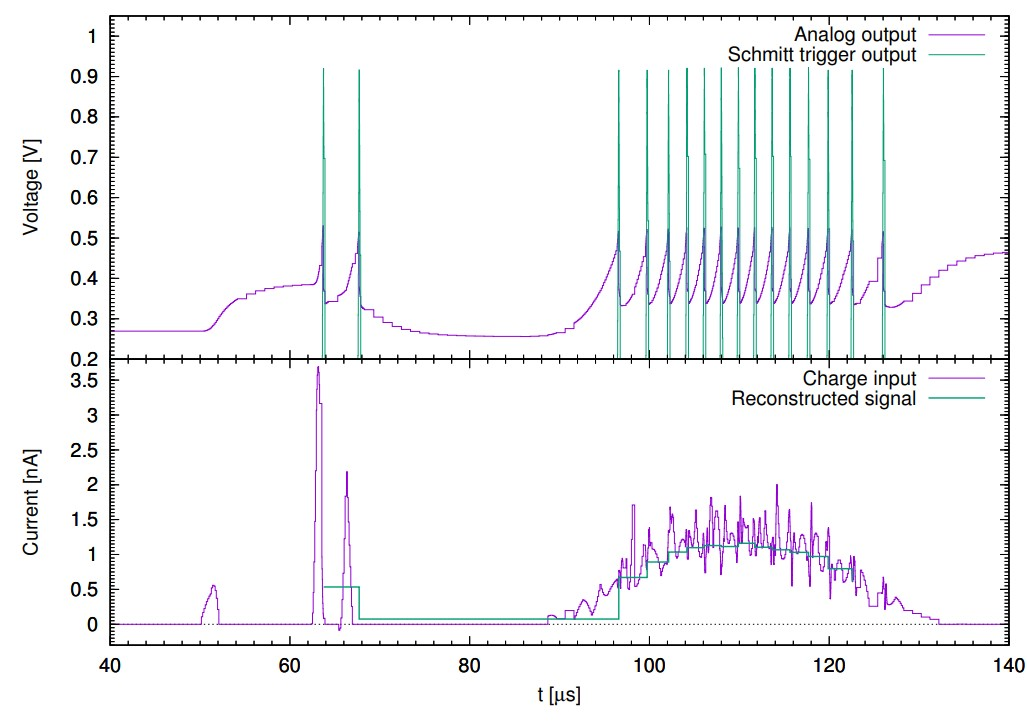
\includegraphics[width=\textwidth]{images/qpix_rtd_reconstruction_example.jpg}
\caption{Example reconstruction of the reset time difference (RTD) based on the Q-Pix readout design. 
Shown is transistor-level charge integration simulation results for minimum ionizing tracks in LAr.
The purple curve of the top pannel represents charge accumulating on the CSA, where the green curve is the reset output from the Schmitt trigger.
The bottom pannel shows input charge (purle curve) overlayed on top of the reconstructed current signal.
The $Q_{o}$ value taken here is equal to 1~\unit{fC}.
Image is taken from \citep{qpix:nygren:mei}.}
\label{fig:qpixRecon1}
\end{figure}

\begin{figure}[]
\centering
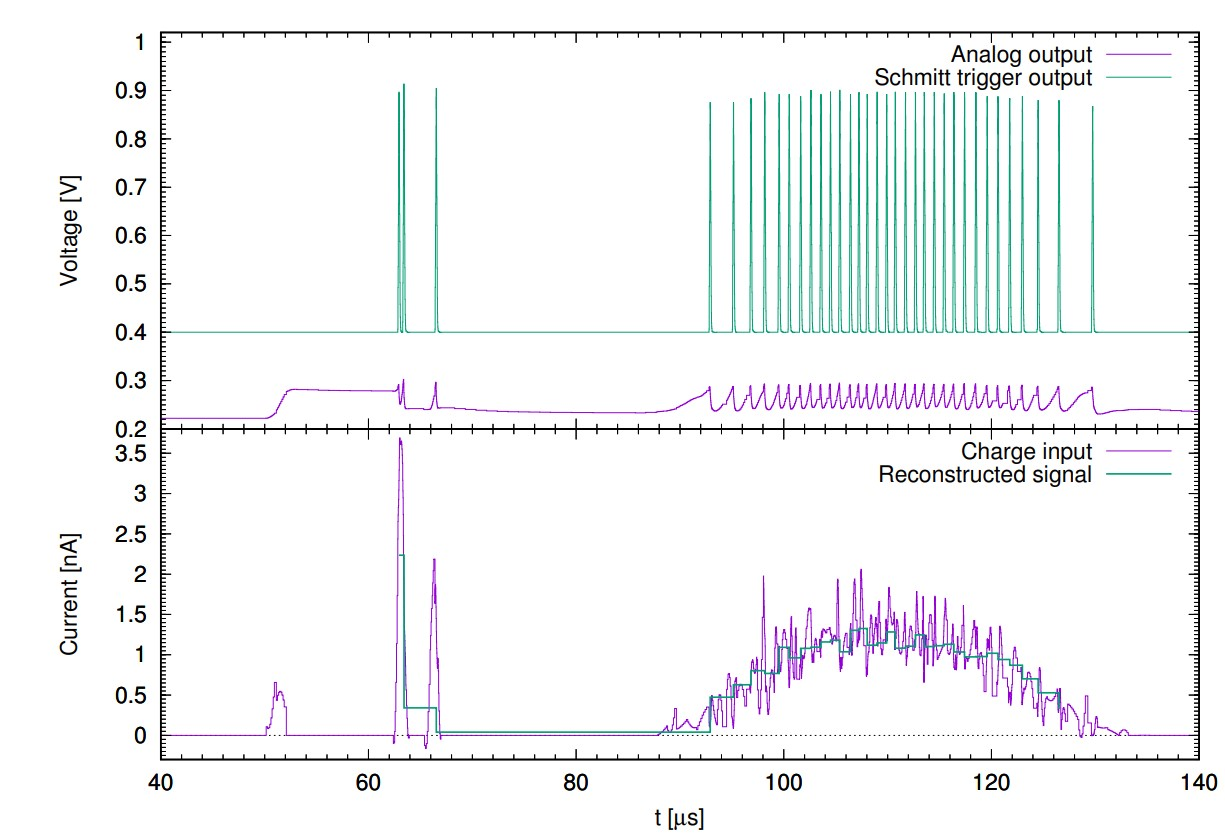
\includegraphics[width=\textwidth]{images/qpix_rtd_reconstruction_example_03fc.jpg}
\caption{Example reconstruction of the reset time difference (RTD) based on the Q-Pix readout design.
Shown is transistor-level charge integration simulation results for minimum ionizing tracks in LAr.
$Q_{o}$ was chosen to be $0.3 fC$.
The bottom panel in this image shows a better match of the reconstructed signal with a smaller $Q_{o}$. 
However, more ($\approx$ 1.0~\unit{fC} / 0.3~\unit{fC}) resets are produced as a result. 
Image is taken from~\citep{qpix:nygren:mei}.}
\label{fig:qpixRecon2}
\end{figure}

Of these three parameters in Equation~\ref{eq:irecon_freq}, two of them need to be calibrated.
The validation of the charge calibration is beyond the scope of this work, but is briefly described in Chapter~\ref{chap:sim} Section~\ref{sec:radiogenic_calib}.
The local oscillator frequency is a digital ASIC level calibration and its results are a product of this thesis.
It's procedure and first results are described in Chapter~\ref{chap:qdb}.
The remaining reconstruction parameter is the timestamp, which is recorded by the digital back-end.

\subsection{Track Reconstruction}

One of the important features of a TPC is the ability to precisely reconstruct full tracks of ionizing particles.
An intended benefit of a pixelated readout on any TPC is to show that there are improvements to reconstruction of these 3-D images.
Event reconstruction requires 3-spatial coordinates (x,y,z) of a track's charge as well as time, t. 
The Q-Pix readout gives two (x,y) coordinates for "free".
Time is intrinsic to the Q-Pix datum, and may also be provided by an external photonics system (see Section~\ref{sec:qpix_photonics}).
The first measured timestamp could also be used as The starting time of any reconstructed track.

The final coordinate, z, is obtained with the LAr drift velocity (Table~\ref{tab:lar_prop}) and the drift time ($t_{drift}$) by the equation:
\begin{equation}~\label{eq:driftDistance}
  z_{drift} = v_{e} * t_{drift}
\end{equation}

The current input onto a pixel calculated from Equation~\ref{eq:irecon_freq}.
If a pixel requires a calibrated $Q_{o}$ to perform a reset, we can relate the charge and current with:
\begin{equation}~\label{eq:piece_wise}
  Q_{i,drift}(t) = \frac{Q_{o}f_{o}}{N_{i,rtd}}t
\end{equation}

The reconstructed charge as a function of time is a piece-wise function of time based on the difference between successive $N_{rtd}(i)$
The slopes of the i-th interval the are given by $\frac{Q_{o}f_{o}}N_{i,rtd}$ Equation~\ref{eq:piece_wise}.
Finally, the charge as a function of position (z position of the charge), is calculated by identifying $t = t_{drift}$ between Equations~\ref{eq:driftDistance} and~\ref{eq:piece_wise}.

\subsection{Comments on Uncertainties}

The verification of the Q-Pix readout, in part, relies on tests to show that these timestamp data can be safely recorded and sent without loss to disc.
Here we briefly discuss potential uncertainties within the Q-Pix readout.

\subsubsection{Near Maximum Reset Rate}

Equation~\ref{eq:irecon_freq} relates the maximum current ($I_{max}$) in a Q-Pix readout at the limiting case of $N_{rtd} = 1$.
For $Q_{o} = 1~\unit{fC}$ and $f_{o} = 30~\unit{MHz}$, $I_{max} = 30~\unit{nA}$.
However, since $N_{rtd}$ is a difference between two 32-bit timestamps, it can only take positive integer values.
This means that each current measurement can only take the form, for N integer: 
$$
I_{max} \sim \frac{30~\unit{nA}}{N}
$$

Therefore, there can be large uncertainty in the measured currents for RTDs near the frequency of the oscillator.
However, if there is sufficient total charge these discrete uncertainties can be accounted for after digital processing.
An example of a periodic artificial input current of with $I \approx I_{max}/10$ is shown below in Figure~\ref{fig:savgol}.
The reconstructed charge over time is shown in Figure~\ref{fig:reconQ}.

\begin{figure}[]
\centering
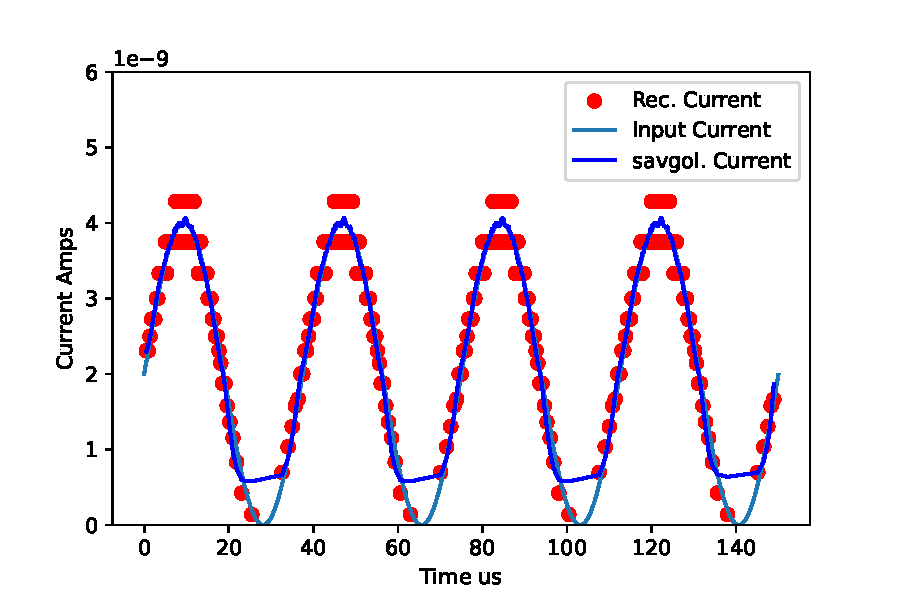
\includegraphics[width=\textwidth]{images/savgol.pdf}
\caption{Arbitrary sine wave based current input.
The maximum amplitude is chosen to be close to $I_{max}$.
Reset Charge is chosen to be 1 $\unit{fC}$ and digital clock frequency of 30 $\unit{MHz}$.
The input current amplitude is close to the maximum, so that the reconstructed current can is far from the actual.
This occurs since $N_{rtd}$ can only take integer values, the recontructed current can only take values of $\frac{30}{N}$.
The red points indicate possible reconstructed current values, where the two highest points correspond to $\frac{30}{7}$ and $\frac{30}{8}$, respectively.
However, an example of a savgol filter (dark blue) is performed on the resets after the fact with near agreement of the large input.
A use case of this kind of digital filtering would be applied to large current values only (peaks of the curves), and not for low current inputs where the pure timestamp difference provides better results.}
\label{fig:savgol}
\end{figure}

\begin{figure}[]
\centering
\begin{subfigure}{.5\textwidth}
  \centering
  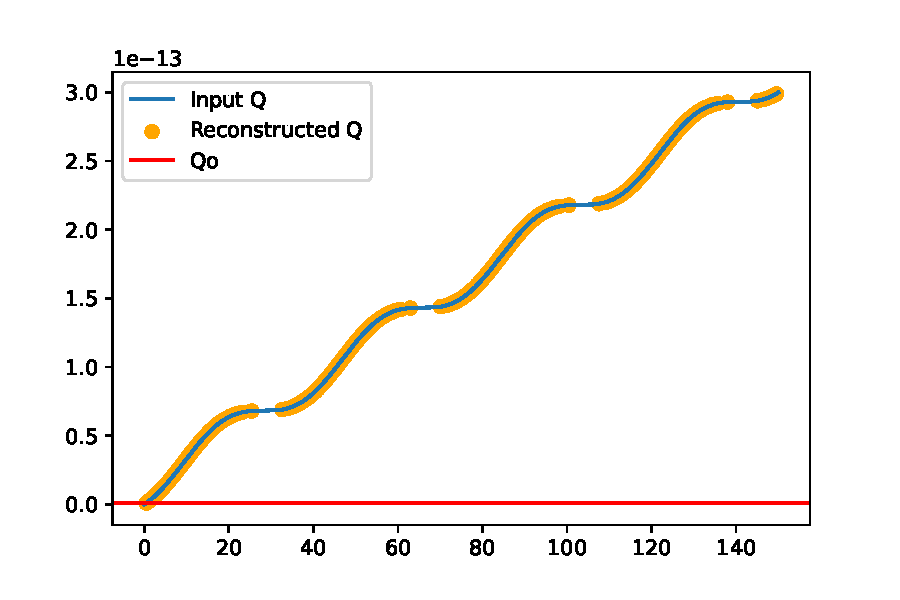
\includegraphics[width=\textwidth]{images/reconQ.pdf}
  \caption{CDF}
\end{subfigure}%
\begin{subfigure}{.5\textwidth}
  \centering
  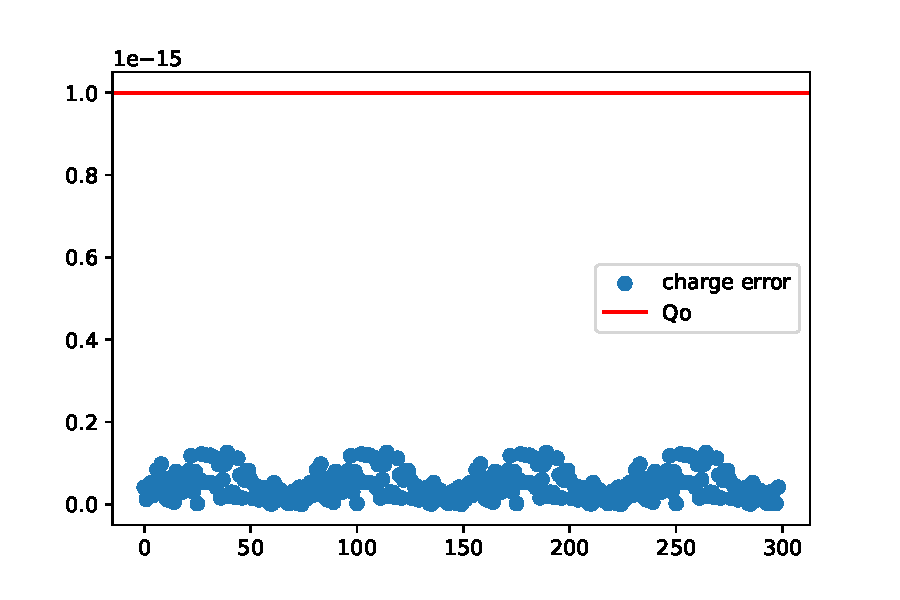
\includegraphics[width=\textwidth]{images/diffQ.pdf}
  \caption{Difference}
\end{subfigure}
\caption{Reconstruction of Sub figures cumulative distribution function (CDF) of charge as a function of time (a) and the error (b).
The input current for these data are showin in Figure~\ref{fig:savgol}.
The pause in resets are when the error is small, since the current input is near zero.
The red line indicates the minimum charge required for a single reset.
The right plot indicates the difference between the true and reconstructed charge distributions compared to a single reset.
}
\label{fig:reconQ}
\end{figure}

\subsubsection{Comments on Reconstruction Requirements}~\label{sec:recon_uncert}

The uncertainty for the two transverse coordinates ($\hat{x}$ and $\hat{y}$) come from the pixel size.
If we assume the electric field to be uniform, on average, across all $\mathcal{O}(10^{7})$ pixels in an APA, then the charge drift will be uniformly distributed over the pixel size.
Then, the pixel dimensions determine the resolution: $\frac{3 mm}{\sqrt{12}} \approx 0.87 mm$.

In order to reach the required uncertainty to measure the z-position ($\sigma_{z} \simeq 1~\unit{mm}$), the uncertainty from $f_{o}$ must be small ($\sim$ 1~\unit{ppm}).
Other measurement uncertainties stem from Equation~\ref{eq:irecon_freq}.
The precision of the local oscillator frequency and the constant charge per reset determine the current reconstruction precision.
Variable replenishment circuits can impace $Q_{o}$, which will also affect $\sigma_{z}$.

\section{How Q-Pix fits into a 10 kt LArTPC}~\label{sec:qpix_apa}

A future target detector for the Q-Pix readout is the DUNE-FD 10 kt module.
To explore how Q-Pix could be used in this detector we provide a brief over-view of the DUNE-FD electronics and compare with those requirements for Q-Pix based readout.
The simulation results presented in Chapter~\ref{chap:sim} are based on the detector volume of a single APA within a DUNE-FD module.

\subsection{The DUNE Far Detector Electronics}

%% section 1.8 of TDR
The DUNE-FD is a modular assembly of Anode Plane Assemblies (APA) as shown in Figure~\ref{fig:dune_apa_tdr}.
Each Single-Phase (SP) 10 kT module consists of 150 APAs.
The APA's full description can be found at~\citep{DUNE-FD_TDRv4:Abi_2020}.
Each APA stores its own the front-end electronics which are in the LAr and are shown in Figure~\ref{fig:dune_tpc_electronics}.

Figure~\ref{fig:dune_tpc_electronics} shows that each APA uses 20 FEMBs to digitize 128 of the 2560 channels.
Of the 128 channels 40 are each taken from the U and V (induction) layers, and 48 wires are taken from the X (conduction) layer.
Each FEMB also houses a total of 18 ASICs which smooth, digitize, and aggregate data before being sent to the Warm Interface CRATE (WIC).
The total number of ASICs per APA is $18\times 20 = 360$.
Since each 10 kt module uses 150 APAs the total number of ASICs would be multiplied by 150.

\begin{figure}[]
\centering
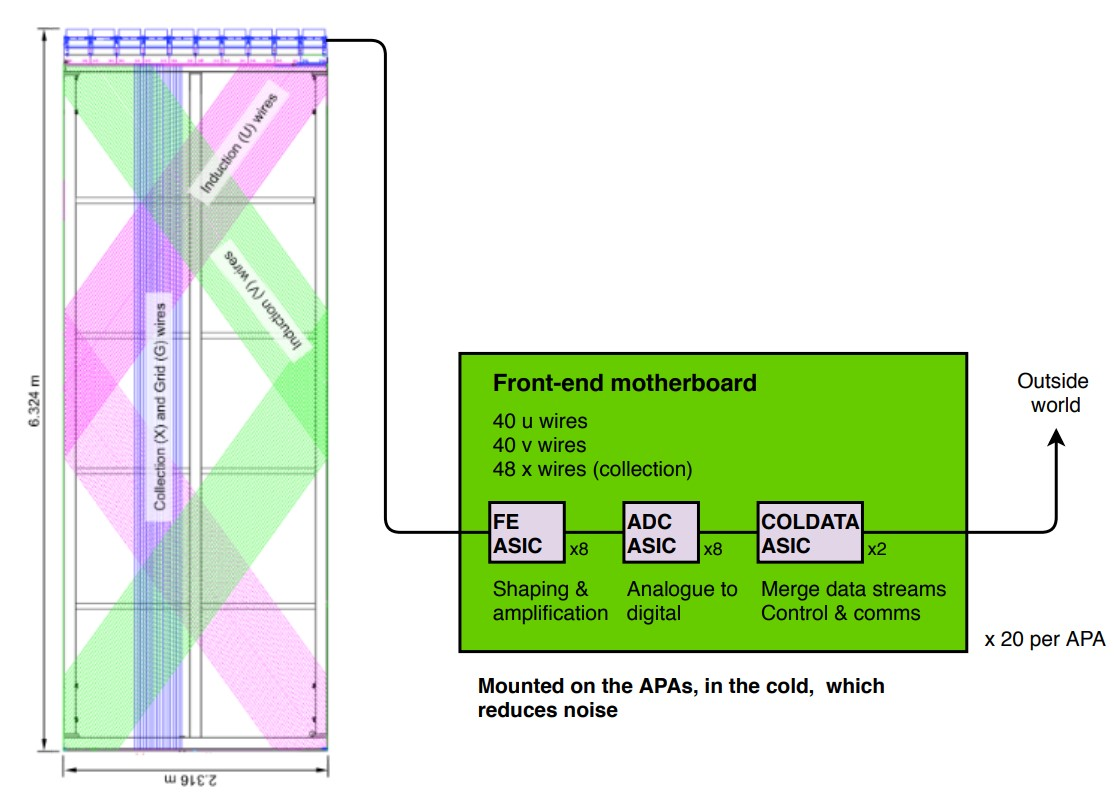
\includegraphics[width=\textwidth]{images/dune_apa_motherboards.jpg}
\caption{Image taken from~\citep{DUNE-FD_TDRv4:Abi_2020}, Fig 1.12 of section 1.8.
Image shows an overlay the the relevant charge collection wires within a DUNE-FD SP LArTPC.
}~\label{fig:dune_tpc_electronics}
\end{figure}

%% example image of DUNE-APA from DUNE-FD TDR.
\begin{figure}[]
\centering
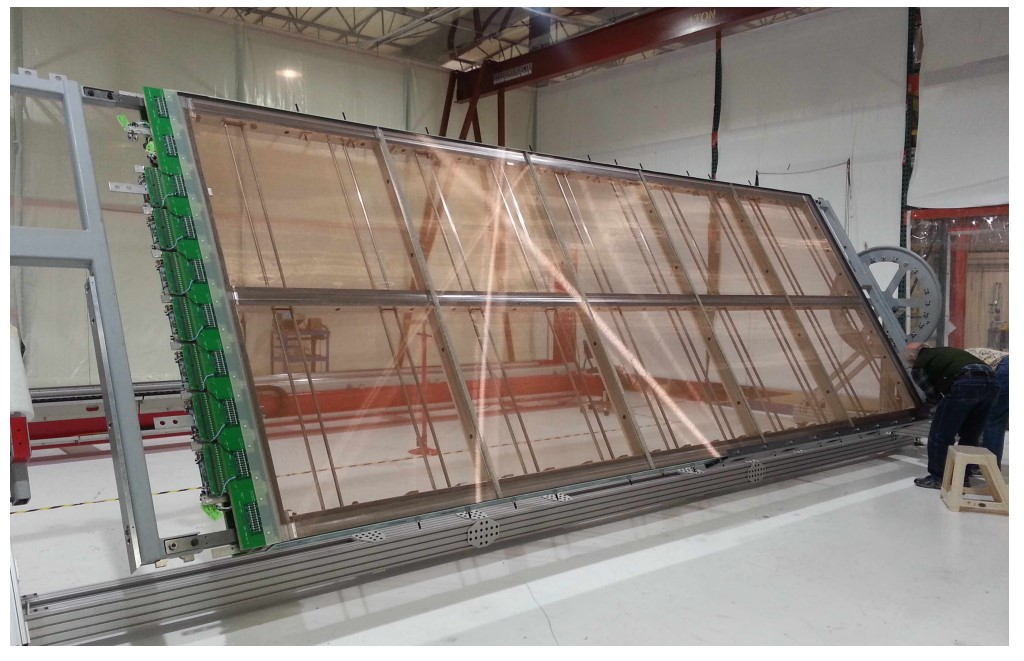
\includegraphics[width=\textwidth]{images/dune_fd_tdr_apa_image.jpg}
\caption{Cross sectional picture of a single DUNE-FD APA backet~\citep{DUNE-FD_TDRv4:Abi_2020}}
\label{fig:dune_apa_tdr}
\end{figure}

On each FEMB are three ASICs are responsible for collecting the charge as it passes between the wires and sending it out of the cryostat.
The first ASIC is a waveform-shaping and amplification ASIC.
The second ASIC is the ADC ASIC and is reponsible for the converting the analog signal to digital.
The final ASIC, called the COLDATA ASIC, merges the data streams from the previous ASICs and is responsible for communication between the motherboard and the outside world.

Table~\ref{tab:dune_tpc_elec} summarizes the electronic requirements expected for the DUNE-FD SP module
The maximum expected data collection is expected to not exceed more than 30 PB/year, which corresponds roughly to $\approx 1 Gb/s$ of continuous collection.
The expected wire electron noise level is design to be $\approx$ 1000 $e^{-}$.
Sampling frequency of 12 bit ADCs is 12 $\unit{MHz}$.
Large signals require a linear reponse of 500 k$e^{-}$, and ensures that fewer than 10\% of beam events experience saturation.
Dune expects to draw less than 50 mW per channel, and incur less than 1\% dead channels.

\begin{table}
\begin{center}
\begin{tabular}{|| p{50mm} | p{40mm} | p{60mm} ||}
 \hline
 Description & Specification & Rationale \\ [0.5ex]
 \hline\hline
  System Noise & < 1000 $e^{-}$ & Provides >5:1 S/N on induction planes for pattern recognition and two-track separation. \\
 \hline
  Signal Saturation & 500,000 $e^{-}$ & Maintain calorimetric performance for multi-proton final state. \\
 \hline
  Cold Electronics Power Consumption & < 50~\unit{mW} per channel & No bubbles in LAr to reduce HV discharge risk\\
 \hline
  Number of Channels per front-end motherboard & 128 &  The total number of wires on one side of an APA, 1,280, must be an integer multiple of the number of channels on the FEMBs. \\
 \hline
  Dead Channels & < 1\% & Minimize the degradation in physics performance over the > 20-year detector operation. \\
 \hline
  Maximum diameter of conduit enclosing the cold cables while they are routed through the APA frame. & 6.35 cm (2.5") & Avoid the need for further changes to the APA frame and for routing the cables along the cryostat walls \\
 \hline
\end{tabular}
\caption{Selected Requirements of DUNE-FD TPC electronics and Expected QPix Design goals of first generation ASIC development for comparison.
The table information is taken from the inner three columns of Table 4.1 in~\citep{DUNE-FD_TDRv4:Abi_2020}.
Due to the different charge sensitive geometries between a wire and pixel-based readout, the required noise and number of channels are not easily comparable.
}
\label{tab:dune_tpc_elec}
\end{center}
\end{table}

\subsection{Q-Pix Comparison to DUNE-FD Electronics}

Each APA is 6.324 $\unit{m}$ $\times$ 2.316 $\unit{m}$, for a total area of 14.646 $\unit{m^{2}}$.
From these dimensions the expected channel count of the QPix readout on the DUNE-FD APA is
\begin{equation}
  N_{pix} = 14.646 m^{2} * \frac{1 pixel}{4 mm^{2}} * \frac{ 1000^{2} mm^{2} }{m^{2}} = 915399
\end{equation}

The total number of free running oscillators ($N_{osc}$) per DUNE-APA for a given pixel pixel of $4~mm^{2}$ is:
\begin{equation}~\label{eq:nosc}
N_{osc} = \frac{915399}{16} \approx 57213
\end{equation}

$N_{osc}$ represents the total number of front-end ASICs whose data must be aggregated and sent outside of the cold electronics to a warm interface.
Therefore we expect the order of the number of free running oscillators per DUNE-APA $\mathcal{O}$($10^5$).
This also gives an order of magnitude estimate of the increase of number of ASICs compared to the MWPC readout of Single-Phase (SP) DUNE-FD.

To have a comparable power draw compared to DUNE-FD, which has 2560 channels, then QPix would need less than $\approx 140 \mu W$ of power draw per channel.
Too much energy disappated in the LAr creates bubbles which is a high voltage (HV) discharge risk.
The total channel count for a 10 kT module is based on 150 DUNE-APAs or $2560\times 150 = 384000$.
Thus, the number of extra analog channels that QPix is required to measure, compared to the typical wire readout, increases by a factor of $915399 / 2560 \approx 357$.

Q-Pix will instead offer conversion from analog (charge) to digital (32 bit time) signals on a single ASIC.
These front-end ASICs would be arrayed in modular tiles within a single APA.
Where the of tiles themselves would be connected and spread out to cover the entire area of an APA.

To connect the entire APA the Q-Pix readout will design modular tiles which will hold a subset of nodes ($\sim$ 16$\times$16 ASICs).
Each tile will interface with a single FPGA (or other ASIC) chip which would concentrate the digital data for each tile; we refer to this FPGA as the DAQ-Node (DN).
Then, each DN can interface could optionally connect a single concentrator FPGA for the entire APA.
This final concentrator would send the data to the Warm-Interface-Cards (WIC) out of the cold electronics (CE).
The final concentrator FPGA we refer to as the Super-DAQ-node (SDN).

The exact description and characteriziation of the WIC for a Q-Pix depends on the final implementation of the SDN.

\begin{table}
\begin{center}
\begin{tabular}{|| p{40mm} | p{40mm} | p{70mm} ||}
 \hline
 Description & Specification & Rationale \\ [0.5ex]
 \hline\hline
  System Noise & $\approx 300 e^{-}$ & Provides $\approx$ 17:1 S/N ratio, a component of front-end integrator. \\
 \hline
  Signal Saturation & 30~\unit{nA} per pixel & Upper limit from local oscillator frequency and integrator reset. \\
 \hline
  Cold Electronics Power Consumption &  $< 100 \unit{\mu W}$ per channel & Equivalent power consumption for heating found in DUNE-FD. \\
 \hline
  Number of Channels per Tile & 4096 &  Design parameter to be calculated. \\
 \hline
\end{tabular}
\caption{Q-Pix based Requirements which are compared to the equivalent DUNE-FD SP module found in table~\ref{tab:dune_tpc_elec}.
Results here are necessarily speculative, but provide an insight to the design goal.
The system noise is a contribution of leakage current per reset, uneven electric fields in the TPC, or uncertainties in the replenishment circuit per reset.
Signal saturation is defined as the maximum measureable current based $Q_{o} = 1~\unit{fC}$ and $f_{o} = 30~\unit{MHz}$.
The Q-Pix readout can also be saturated by too many resets if the FIFO buffers overflow (see Chapter~\ref{chap:sim} for further discussion).
The power consumption per channel is a direct division compared to Table~\ref{tab:dune_tpc_elec}.
The number of channels per tile depends on the tile size as well as the number of pixels per ASIC (see Chapter~\ref{chap:qdb} for further discussion).
}
\label{tab:qpix_tpc_elec}
\end{center}
\end{table}

\section{The Digital Back-end}~\label{sec:digital_back-end}

We define the digital back-end as the part of the larger Q-Pix readout system that is responsible for handling the timestamp data once it is recorded.
This sub-system must be able to record and store data, be robust against SPF, define error states, and more.

In this section we introduce considerations which guided the design of the first two Q-Pix ASIC prototypes.
These design choices for the digital prototype are enumerated in table~\ref{table:digital_design_params}.

\subsection{Digital ASIC Prototype Desgin Choices}~\label{sec:design_choices}

The Table~\ref{table:digital_design_params} highlights some design choices of the first digital Q-Pix ASIC prototype.
Four neighbor connections were chosen as the design choice two allow for communiation in either direction along the x and y axes.
The local and remote FIFO depths determine how many resets and communication packets the ASIC may store at any one time.

\begin{table}
\begin{center}
\begin{tabular}{||p{30mm} | p{30mm} | p{90mm}||}
 \hline
 Parameter Name & Value & Description \\ 
 \hline\hline
Local Oscillator Frequency & 30~\unit{MHz} & Determines maximum current reconstruction (Equation~\ref{eq:irecon_freq}). Stability of local oscillator also determines z-position reconstruction uncertainty (Sect.~\ref{sec:recon_uncert}). \\
 \hline
Connections & 4$\times$2 (Tx and Rx) &  Eight differential pair connections are made to support four transmitter (Tx) and receiver (Rx) lines. \\
 \hline
Communication Protocol & Endeavor & Protocol determines packet stability based on oscillator frequency as well as packet transaction time. Results of these tests are done in Chapter~\ref{chap:qdb}. \\
 \hline
Timestamp Bits & 32 & Determines the total number of unique counts each timestamp value can take. Also determines the "wrap-around" time based on the local oscillator.  \\
 \hline
Local FIFO Depth & 64 & Total number of timestamps the ASIC can store before running out of memory. ASIC will not record additional resets until emptied. \\
 \hline
Remote FIFO Depth & 128 & Total number of remote packets ASIC can store before running out of memory. ASIC will not write additional packets from neighbors. \\
 \hline
 \hline
\end{tabular}
\caption{Summary of design parameters for the first Q-Pix digital ASIC.
The local oscillator is a ring oscillator with a targeted mean of 30~\unit{MHz}.
Each ASIC will be able to communicate with up to four neighbor nodes via a custom "Endeavor" protocol.
The testing and verification of the endeavor protocol is found in Chapter~\ref{chap:qdb}.
The values of the local and remote FIFO depth were selected due to fabrication requirements, whose future values are discussion of Chapter~\ref{chap:sim}.
}
\label{table:digital_design_params}
\end{center}
\end{table}

\subsection{Single Point Failures}

Q-Pix digital design should provide  ``robust resilience'' against single point failure (SPF).
The readout technology presented here relies on huge numbers of readout channels ($10^{8}$) compared to current MWPC designs ($10^{5}$).
As such, extra care must be made in designing new technology to improve over established, seemingly simpler means.

This principal guides design choices such as the use of independent local oscillators at the pixel-level instead of a provided distributed clock.
This design choice, in particular, is discussed at length in Chapter~\ref{chap:qdb}, and the findings presented there are one of the major contributions presented in this thesis.

The design which avoids SPF and handles the digital requirements presented here, namely: the continual time calibration of each local oscillator ($N_{osc} \approx 10^{5}$) is a product of this thesis.
However, the amount of data produced depends on the charge collected in each event, therefore the amount of data collected can not be known before recording.

\section{Q-Pix and Light Detection}~\label{sec:qpix_photonics}

The results of this thesis analyze the response of the Q-Pix digital readout without any analysis paid towards photon collection.
However, recent progress regarding amorphous selenium (aSe)~\citep{https://doi.org/10.48550/arxiv.2207.11127} has been made towards inclusion of an optical system.

The current pixel dimensions of Q-Pix are 4 $\unit{mm}$ $\times$ 4 $\unit{mm} $ which have a total active area of 16$\unit{mm^{2}}$.
Most of this active area is unused for the charge collection pad, which could be as small as drill-hole via (6 mil $<<$ 16\unit{mm^2}).
Most of the remaining area, then, could be plated with a photo-sensitive material (such as aSe).

aSe could capture incoming scintillation photons and provide an additional voltage measurement at each pixel.
Depending on the sensitivity, such a measurement could be used to reconstruct tracks by providing a $\frac{dE}{dX}$ measurement, or even be used as a time-tag or a trigger.

The use of a reference trigger could be useful to establish event-time within the same system, and allow adjacent pixels which would receive photons, but not charge, to contribute to time reconstruction.
Any reconstructed event requires some $T_{o}$ time to indicate the start of the event.
Typically this is done via scintillation photons from a secondary system, where the photons arrive nearly instantly at the collection planes compared to the slow drift speed of the electrons.

The natural pixelization of Q-Pix required the charge collection can also be used to be sensitive to scintillation photons.
These photons could not only provide the required event timing but also provide an additional means of calorimetry and track reconstruction.
Additional work is currently underway to demonstrate the viability.

Currently there are two competing geometries to incorporate light collection within Q-Pix.
Figure~\ref{fig:qpix_light_geometries} shows the vertical and horiztontal drift geometries.
The vertical drift geometry is an easier design geometry, however the top electrode must not only be able to collect charge it must also be transparent. 
On the other hand, the horizontal drift geometry solves the transparancy problem but involves a more complilcated hardware design. 

\begin{figure}[]
\centering
\begin{subfigure}{.45\textwidth}
  \centering
  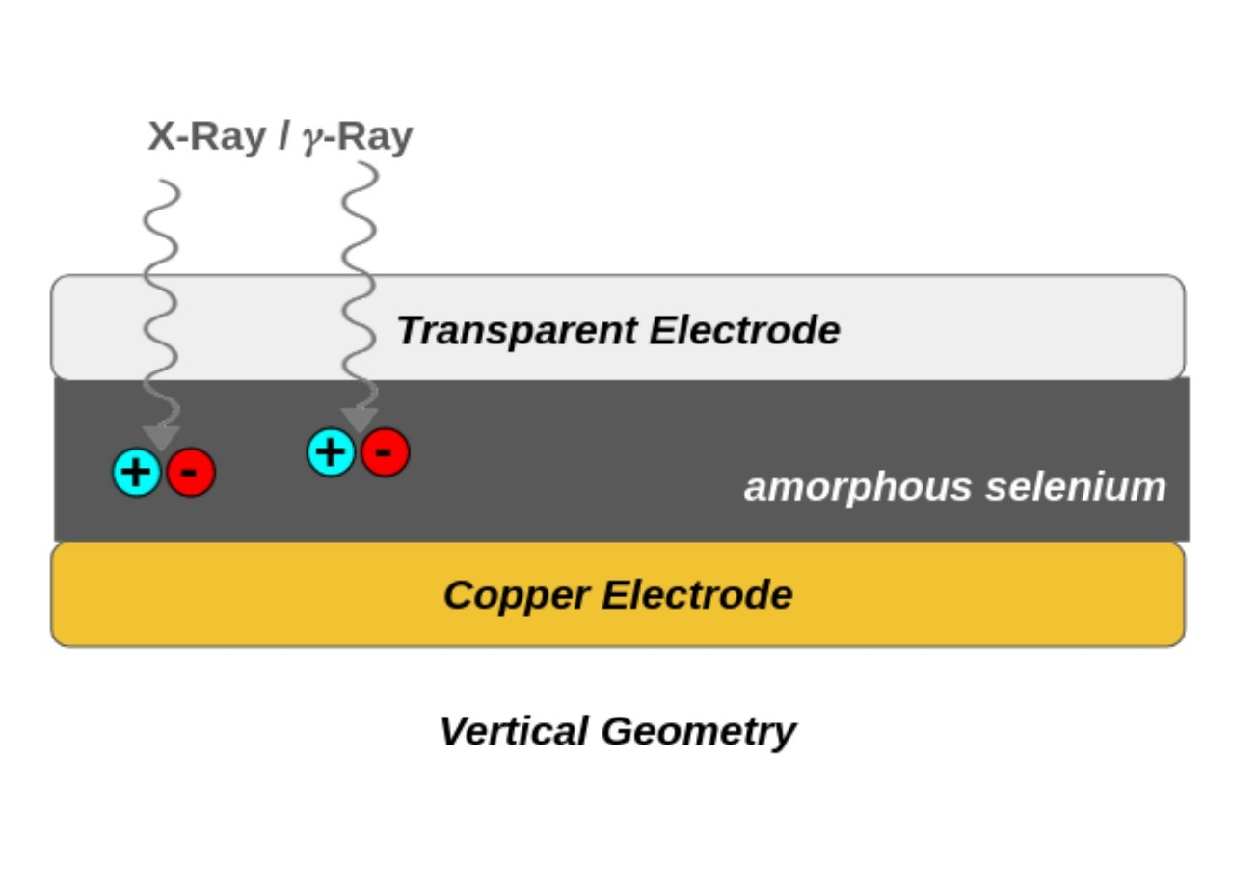
\includegraphics[width=\textwidth]{images/qpix_light_vertical_geom.pdf}
  \caption{Vertical Drift}
\end{subfigure}%
\begin{subfigure}{.45\textwidth}
  \centering
  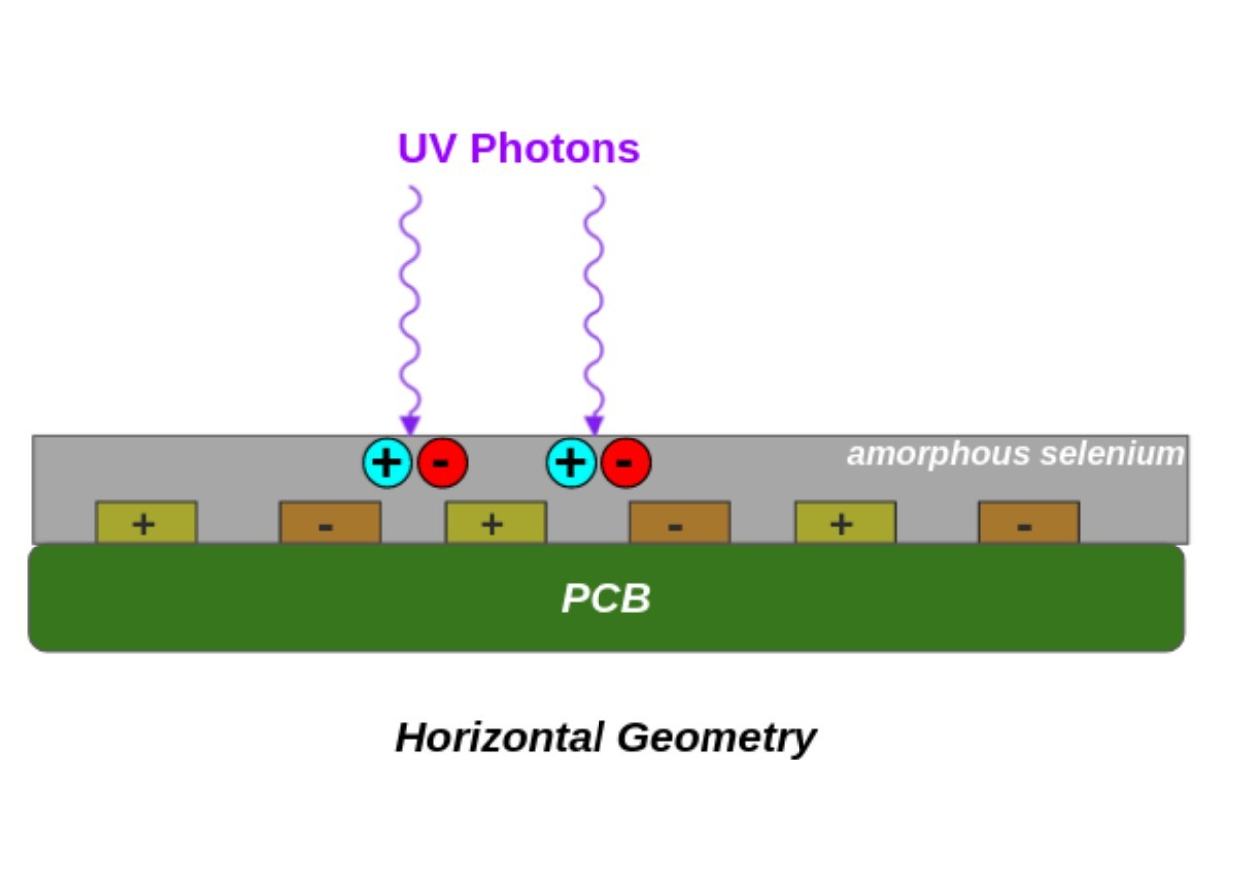
\includegraphics[width=\textwidth]{images/qpix_light_horizontal_geom.pdf}
  \caption{Horizontal Drift}
\end{subfigure}
\caption{Images taken from~\citep{https://doi.org/10.48550/arxiv.2207.11127}.
The vertical drift geometry (left) shows an electrode on the top layer, whereas the horiztontal (right) geometry integrates the electrodes within the aSe.
The vertical geometry is an easier design, but most electrodes are not transparent to VUV scintillation light.
The horiztontal geometry solves this problem, at the cost of a more complicated design.
}
\label{fig:qpix_light_geometries}
\end{figure}

\section{Q-Pix at Low Energy: Supernova Studies}~\label{sec:qpix_supernova}

Work has been done to characterize a Q-Pix readout ability measure core collapse supernovae~\citep{qpix:shion} events within a DUNE-FD module.
These studies involved particle Geant4-based(~\citep{geant4:AGOSTINELLI2003250}) simulations for low energy ($\simeq$ 10~\unit{MeV}) neutrino events.
The results indicate several advantages Q-Pix readout will have over a traditional wire-based readout.

One advantage is the lower overall data rates (1.03$*10^{-6}$ < 2~\unit{pB} per year) compared to the traditional single-phase readout.
This reduction in data rates could allow for a 10 kT Q-Pix module to collect timestamp data continually.
Such a continuous readout, with no trigger, could be particularly useful in collecting supernova burst events.
Figure~\ref{fig:qpix_shion} compares the trigger sensitivity supernova trigger burst effeciencies between the Q-Pix readout against traditional wire-readout. 

\begin{figure}[]
\centering
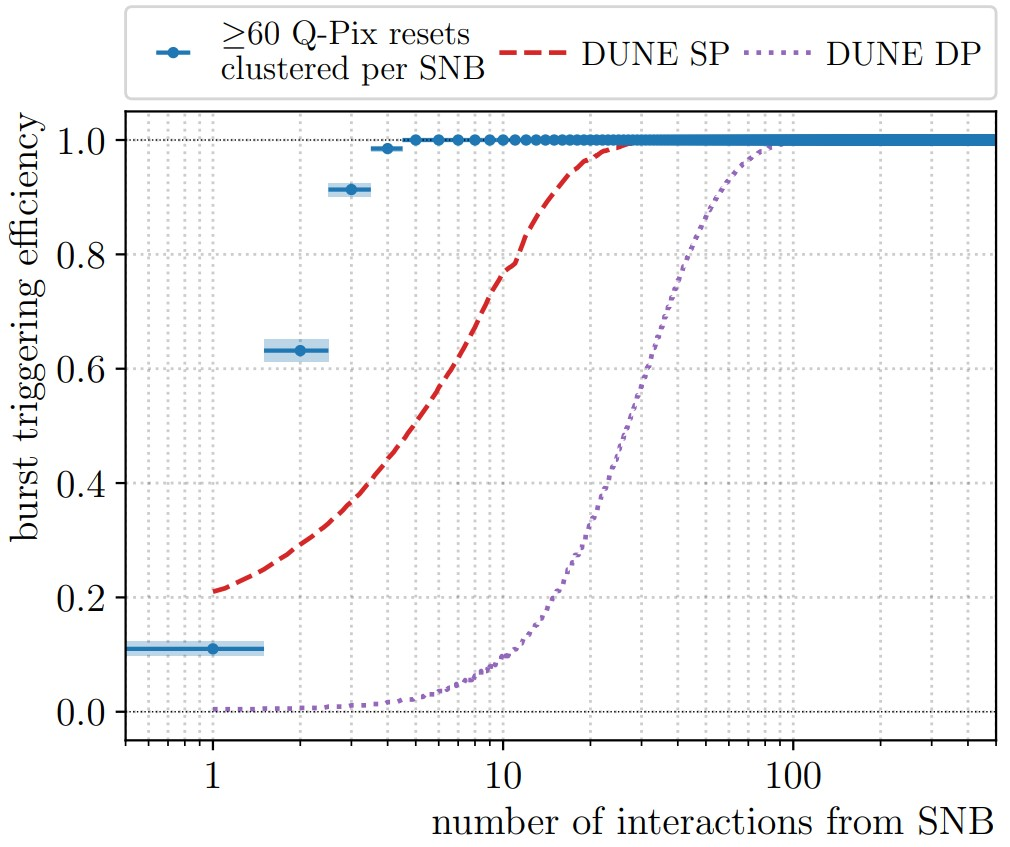
\includegraphics[width=0.6\textwidth]{images/shion_qpix_snb_trigger.jpg}
\caption{Image is taken direclty from~\citep{qpix:shion}.
Plotted is the supernova burst triggering effeciency as a function of $\nu_{e}$ interactions in a 10 kT DUNE-FD module.
The points in blue indicate that a series of 60 resets are "clustered" to use as an identification of a supernova event. 
The other curves are taken from Ref.~\citep{supernova_Abi_2021}.
}
\label{fig:qpix_shion}
\end{figure}